\subsection{Представление данных на диске}
\label{sec:optimization:data_repr}

Для наглядности и простоты в данном примере используем простую схему и ограничимся тем, что \lstinline{sku}, \lstinline{store}, \lstinline{week} имеют каждый ровно 9
записей:

\begin{lstlisting}[language=Prolog]
sku(s), sku_id(s:id) -> string(id).
loc(l), loc_id(l:id) -> string(id).
week(w), week_id(w:id) -> string(id).
sales[s, l, w]=f -> sku(s), loc(l), week(w), decimal(f).
\end{lstlisting}

Исходя из наших ограничений ключами в sales являются трехразрядные числа: 121, 152. Теперь расссмотрим на рисунке \ref{fig:optimization:data_repr:pages_in_memory}, как записи каждого предиката хранятся с помощью страниц.

\begin{figure}
	\centering
	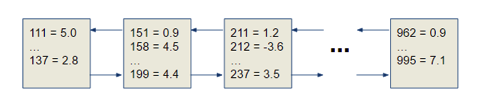
\includegraphics[scale=1.8]{pages_in_memory.png}
	\caption{Пример представления страниц в памяти}
	\label{fig:optimization:data_repr:pages_in_memory}
\end{figure}

Каждая страница хранит упорядоченную последовательность пар ключ/значение. Кроме того, в ней содержатся указатели на следующую и предыдущую страницы для упрощения сканирования страниц. При этом для них необязательно (и в общем случае такое не выполняется) находиться в последовательных блоках памяти и заполненными максимальным количеством пар. Как видно из рисунка, каждая страница в нашем примере содержит лишь значения для одного \lstinline{sku}, поскольку начинаются элементы лишь с определенной цифры, которая по своему месту соответствует как раз параметру \lstinline{sku}.

Эффективной структурой поиска по узлам с помощью таких ключей и указателей является не что иное, как \emph{B+ дерево}, в котором листьями являются страницы с парами ключ/значение. Для краткости и простоты понимания показан лишь один не листовой узел, но в реальности это тоже отдельная страница на диске (на рисунке \ref{fig:optimization:data_repr:page_pointers} горизонтально показана для простоты чтения).

\begin{figure}
	\centering
	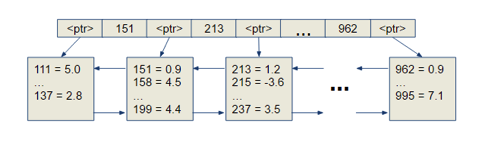
\includegraphics[scale=1.8]{page_pointers.png}
	\caption{Пример использования страницы с указателями}
	\label{fig:optimization:data_repr:page_pointers}
\end{figure}

Теперь посмотрим на запрос:

\begin{lstlisting}[language=Prolog]
_[]=m <-
  agg <<m=max(v) >>
    sku_id(s:"Sprite"),
    loc_id(l:"Belarus")
    sales[s, l, _]=v.
\end{lstlisting}

\lstinline{sku_id}: 1 = \lstinline{Sprite}, ... 9 = \lstinline{Chupa Chups}

\lstinline{store_id}: 1 = \lstinline{USA}, ... 5 = \lstinline{Belarus}, ... 9 = \lstinline{Russia}

Если рассматривать выполнения поиска по шагам:

\begin{enumerate}
  \item инициализируем \lstinline{sku_id} итератор;
  \item двигаем итератор \lstinline{sales} для выравнивания с итератором \lstinline{sku_id};
  \item инициализируем итератор \lstinline{loc_id};
  \item двигаем итератор \lstinline{sales} для выравнивания с итератором \lstinline{loc_id};
  \item считаем агрегированное значение из запроса.
\end{enumerate}
